\documentclass[12pt]{article}
\usepackage[a4paper,margin=0.75in]{geometry}
\usepackage[utf8]{inputenc}
\usepackage[OT1]{fontenc}
\usepackage[table,usenames,dvipsnames]{xcolor}
\usepackage{array}
\usepackage{varwidth}
\usepackage{tabularx}
\usepackage{amsmath}
\usepackage{hyperref}
\usepackage{enumitem}
\usepackage{graphicx}
\usepackage{tcolorbox}
\renewcommand*\familydefault{\sfdefault}

\newtcolorbox{mybox}[3][]
{
  colframe = #2!25,
  colback  = #2!10,
  coltitle = #2!20!black,  
  title    = {#3},
  #1,
}

\hypersetup{
    colorlinks=true,
    linkcolor=blue,
    filecolor=magenta,      
    urlcolor=cyan,
    pdftitle={Overleaf Example},
    pdfpagemode=FullScreen,
}

\title{\textbf{COL774 Assignment 1}}
\author{Aniruddha Deb \\ \texttt{2020CS10869}}
\date{September 2022}

\begin{document}

\maketitle

\section*{Linear Regression}

\begin{enumerate}[label=(\alph*)]
    \item The parameters we used were:
    \begin{itemize}
        \item Learning rate $\eta = 0.01$
        \item Convergence limit $\epsilon = 0.0001$
        \item Final set of parameters: $(\theta_0,\theta_1) = (0.00561383,0.6451277)$
    \end{itemize}

    \item \begin{center}\raisebox{-.9\height}{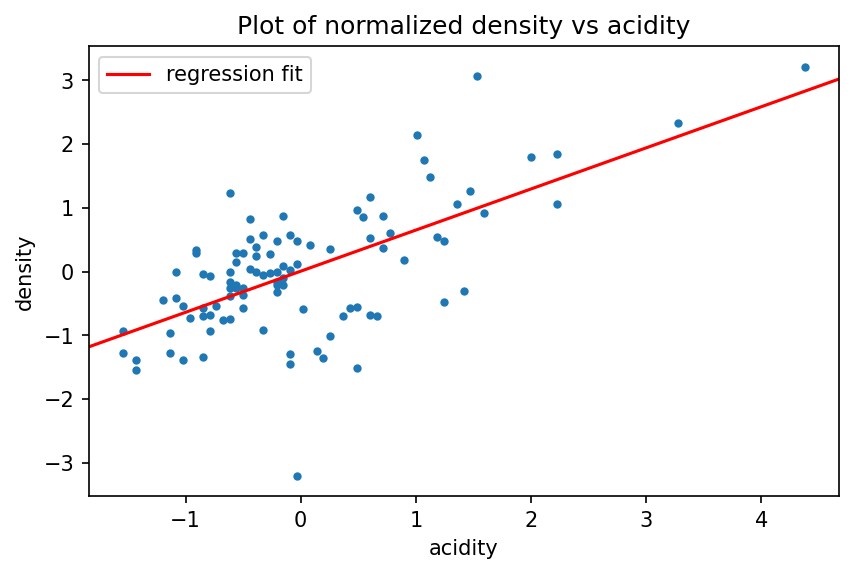
\includegraphics[width=0.7\textwidth]{../Q1/plots/b_plot.png}}\end{center}

    \clearpage

    \item \begin{center}3D mesh plot of gradient, and the path taken by gradient descent ($\eta = 0.01$): \raisebox{-.9\height}{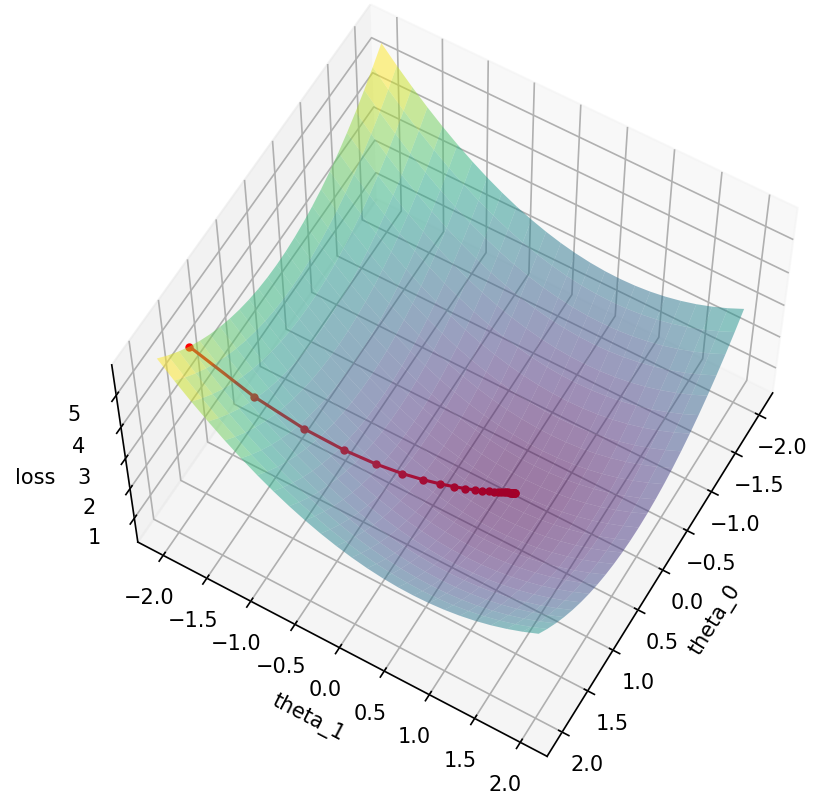
\includegraphics[width=0.7\textwidth]{../Q1/plots/c_mesh.png}}\end{center}

    \item \begin{center}2D contour plot of gradient, and the path taken by gradient descent ($\eta = 0.01$): \raisebox{-.9\height}{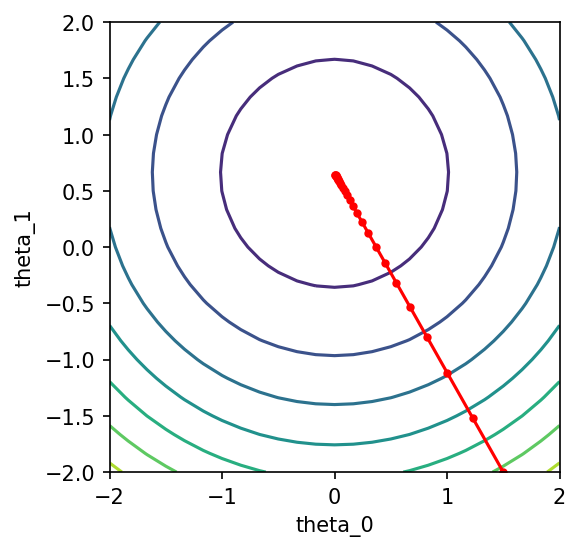
\includegraphics[width=0.7\textwidth]{../Q1/plots/d_contour.png}}\end{center}

    \clearpage

    \item Paths taken by Gradient Descent for varying values of $\eta$: 
    
    \begin{tabular}{c c c}
        $\eta = 0.001$ & $\eta = 0.025$ & $\eta = 0.1$ \\
        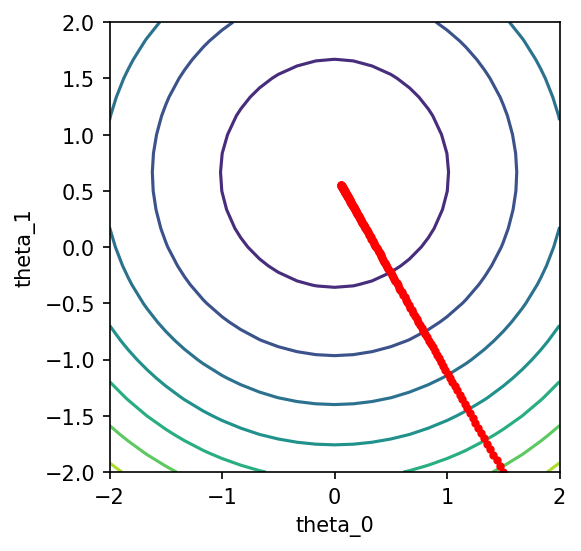
\includegraphics[width=0.3\textwidth]{../Q1/plots/e_contour_001.png} &
        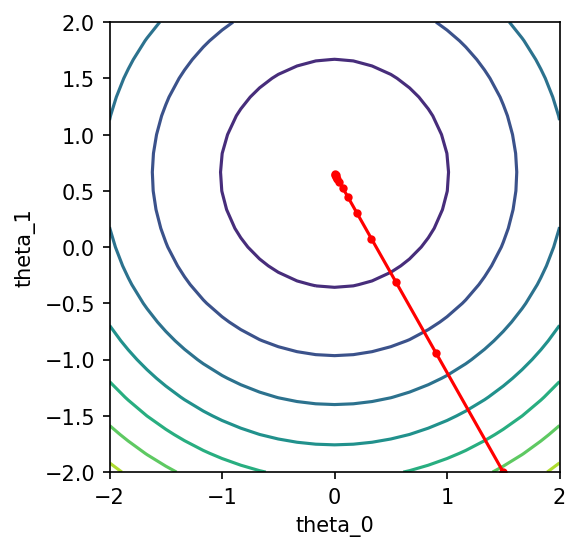
\includegraphics[width=0.3\textwidth]{../Q1/plots/e_contour_025.png} &
        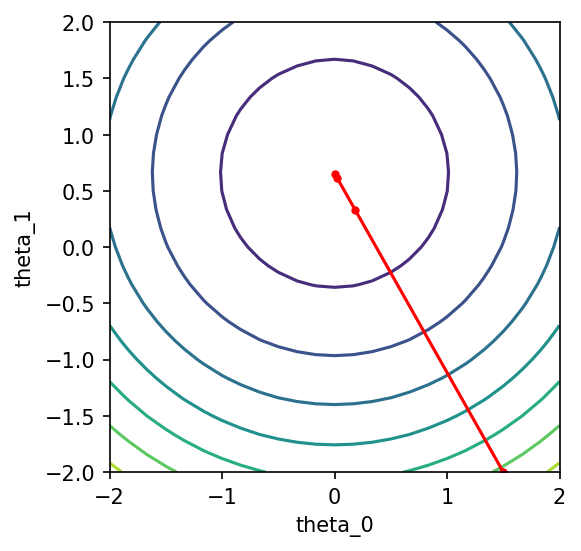
\includegraphics[width=0.3\textwidth]{../Q1/plots/e_contour_1.png} \\
    \end{tabular}

    We notice that with a smaller step size, fewer steps are required to reach convergence; this is beneficial in this case, but can also lead to gradient descent overshooting/not converging in some cases.

\end{enumerate}

\clearpage

\section*{Stochastic Gradient Descent}

\begin{mybox}{LimeGreen}{On Convergence of SGD}
From the video shared, it was suggested that to examine the convergence, loss functions averaged over atleast a 1000 examples be plotted during Stochastic Gradient Descent. A plot over different batch sizes gives the following:

\begin{center}
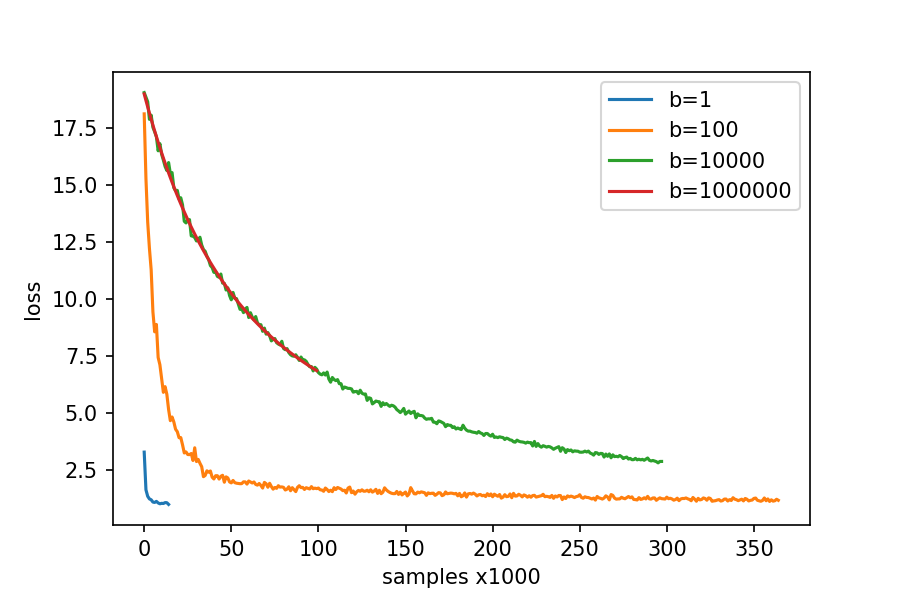
\includegraphics[width=0.7\textwidth]{../Q2/plots/loss.png}
\end{center}

We see that for $b=10^4$ and $b=10^6$, the algorithm does not converge as the learning rate is too low, and the cutoff condition stops it early. As a result, we also include an absolute loss cutoff for learning: stop when the averaged loss over 1000 examples is less than 1.\\

This example shows how to find such a window, given that we don't know the parameters that SGD will converge to: we manually examine the graphs and see what values our converging loss functions are reaching. The graph for $b=1$ and $b=100$ reaches values marginally under 1 (0.97), hence we choose 1 as our cutoff.
\end{mybox}

\begin{mybox}{red}{Note}
We choose to keep the maximum number of epochs at 100, as for $b=10^6$, the slow algorithm was not converging on my machine even after running it for $\approx$5 minutes.
\end{mybox}

\begin{enumerate}[label=(\alph*)]
    \addtocounter{enumi}{1}
    \item With the following convergence conditions:
    \begin{itemize}
        \item number of epochs $t \le 100$
        \item relative difference averaged over (atleast) past 1000 examples $\mathcal{J}^{t+1}_{\ge 1000} - \mathcal{J}^{t}_{\ge 1000} < r_d$
        \item absolute loss function averaged over (atleast) past 1000 examples $\mathcal{J}_{\ge 1000} < 1$
    \end{itemize}

    We obtain the following convergence(s):

    \begin{center}
    \begin{tabular}{|l|l|l|l|l|}
        \hline
        $b$     & $r_d$ & $\theta$ & Time & Batches \\
        \hline
        1       & 0.01  & $(3.03,1.03,2.03)$ & 2.46 s & 88000 \\
        100     & 0.001 & $(2.72,1.06,1.98)$ & 0.24 s & 8520 \\
        10000   & 0.001 & $(2.69,1.07,1.98)$ & 10.80 s & 8122 \\
        1000000 & 0.001 & $(0.25,0.91,0.46)$ & 14.33 s & 100 \\
        \hline
    \end{tabular}
    \end{center}

    \item All the training examples converge close to the actual parameters, except $b=10^6$, as it hits the epoch limit. $b=100$ converges the fastest. $r_d$ for 1 was taken to be $0.01$ as for $b=1$, we get strong oscillations around the local minima (as will be visible in fig. (d)). Other parameters don't converge exactly to the local minima as their averaged loss functions reach below 1 sooner, and as they move slowly, the second condition of relative difference is also satisfied once they get very close to the minima. 

    For the test dataset with 10,000 examples, the loss values are as follows:

    \begin{center}
    \begin{tabular}{|l|l|}
        \hline
        $b$     & $\mathcal{J}(\theta)$ \\
        \hline
        1       & 1.05 \\
        100     & 1.21 \\
        10000   & 1.25 \\
        1000000 & 121.0 \\
        \hline
    \end{tabular}
    \end{center}

    \item \begin{center}\raisebox{-.9\height}{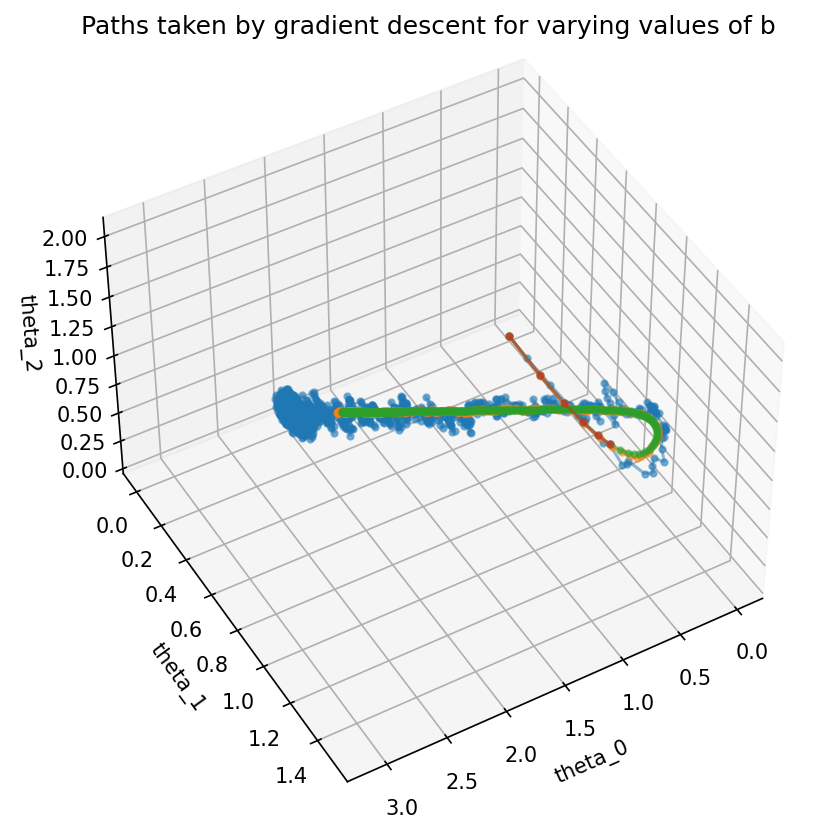
\includegraphics[width=0.7\textwidth]{../Q2/plots/d_paths.png}}\end{center}

    Notice that for $b=1$, the algorithm does not converge to the minima, but instead oscillates in a ball around the minima. This is fixed by taking a variable learning rate (as seen in the video). The other movements are slower, and the red line stops early because it's cut off by the epoch time.

\end{enumerate}

\pagebreak

\section*{Logistic Regression}

\begin{enumerate}[label=(\alph*)]
    \item We obtained the hessian as 
    \begin{align*}
        H(\theta) = \left[ \sum_{i=1}^m -\sigma(\theta^T x^{(i)})(1-\sigma(\theta^T x^{(i)})) x_j^{(i)}x_k^{(i)} \right]_{j,k}^n
    \end{align*}

    Optimizing this via newton method for 1000 iterations, we obtained $\hat{\theta} = (0.26,2.25,-2.23)$

    \item \begin{center}\raisebox{-.9\height}{\includegraphics[width=0.7\textwidth]{../Q3/plots/b_scatter.png}}\end{center}

\end{enumerate}

\pagebreak

\section*{Gaussian Discriminant Analysis}

\begin{enumerate}[label=(\alph*)]
    \item Running GDA on the normalized data gives us 
    \begin{align*}
        \phi &= 0.5 \\
        \mu_0 &= (-0.134,0.217) \\
        \mu_1 &= (0.134,-0.217) \\
        \Sigma &= 
        \begin{bmatrix}
            0.014 & -0.001 \\
            -0.001 & 0.053
        \end{bmatrix}
    \end{align*}

    \item \begin{center}\raisebox{-.9\height}{\includegraphics[width=0.7\textwidth]{../Q4/plots/b_scatter.png}}\end{center}

    \item For the same covariance matrix, the separator is a normal to the line joining the two means, passing through the point $\mu_0(1-\phi) + \mu_1\phi$

    In this case, since the number of datapoints in both classes are equal ($\phi = 0.5$) the separator is simply the perpendicular bisector.

    \begin{center}\raisebox{-.9\height}{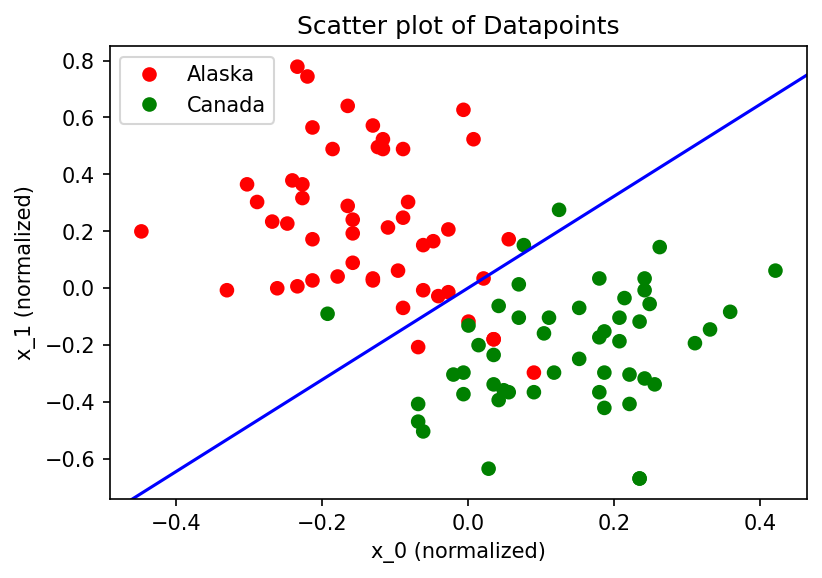
\includegraphics[width=0.7\textwidth]{../Q4/plots/c_lin_boundary.png}}\end{center}

    \item Running GDA for two separate covariances on the normalized data gives us 
    \begin{align*}
        \phi &= 0.5 \\
        \mu_0 &= (-0.134,0.217) \\
        \mu_1 &= (0.134,-0.217) \\
        \Sigma_0 &= 
        \begin{bmatrix}
            0.012 & -0.009 \\
            -0.009 & 0.065
        \end{bmatrix} \\
        \Sigma_1 &= 
        \begin{bmatrix}
            0.015 & 0.006 \\
            0.006 & 0.042
        \end{bmatrix}
    \end{align*}

    \item The quadratic boundary obtained is as follows: 

    \begin{center}\raisebox{-.9\height}{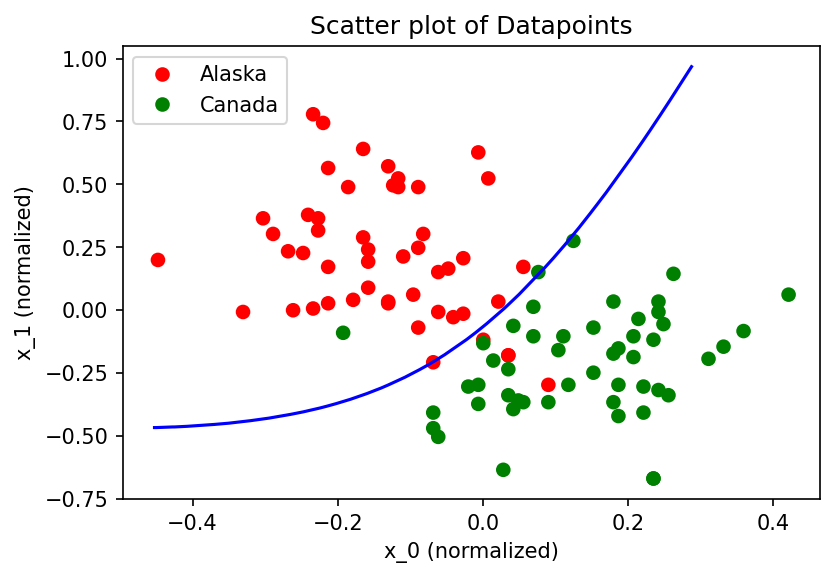
\includegraphics[width=0.7\textwidth]{../Q4/plots/e_quad_boundary.png}}\end{center}

    \item The quadratic decision boundary is better at classification than the linear one: there are only 4 misclassifications in the quadratic classifier compared to 7 in the linear.

    The quadratic decision boundary in this case is a \textbf{hyperbola}, as from \href{https://engineering.purdue.edu/ChanGroup/ECE595/files/chapter2.pdf}{Chan} Pg. 24, we see that if $\Sigma_0^{-1} - \Sigma_1^{-1}$ has one negative eigenvalue and one positive eigenvalue, the separator will be hyperbolic. In this case, the eigenvalues come out to be $34.6$ and $-20.4$, implying that the decision boundary is a hyperbola.

\end{enumerate}


\end{document}
